\documentclass[a4paper,11pt]{article}

\usepackage{geometry}
\usepackage{listings}
\usepackage{mathrsfs}
\usepackage[font={small},labelfont={sf,bf}]{caption}
\usepackage{color}
\usepackage{amssymb}
\usepackage[utf8]{inputenc}
\usepackage{afterpage}
\usepackage[T1]{fontenc}
\usepackage{amsfonts}
\usepackage{mathtools}
\usepackage{amsmath}
\usepackage{verbatim}
\usepackage{bm}
\usepackage{bbm}
\usepackage{enumerate}
\usepackage{amsthm}
\usepackage{stmaryrd}

\geometry{a4paper,top=3cm,bottom=3cm,left=2cm,right=2cm,heightrounded, bindingoffset=5mm}

\theoremstyle{definition}
\newtheorem{definition}{Definition}[section]
\theoremstyle{plain}
\newtheorem{theo}[definition]{Theorem}
\newtheorem{prop}[definition]{Proposition}
\newtheorem{lemma}[definition]{Lemma}
\newtheorem{cor}[definition]{Corollary}
\newtheorem{ex}[definition]{Example}
\theoremstyle{remark}
\newtheorem{rem}[definition]{Remark}
\newtheorem{rem*}[definition]{}

\newcommand*\mcup{\mathbin{\mathpalette\mcupinn\relax}}
\newcommand*\mcupinn[2]{\vcenter{\hbox{$\mathsurround=0pt
  \ifx\displaystyle#1\textstyle\else#1\fi\bigcup$}}}
\newcommand*\mcap{\mathbin{\mathpalette\mcapinn\relax}}
\newcommand*\mcapinn[2]{\vcenter{\hbox{$\mathsurround=0pt
  \ifx\displaystyle#1\textstyle\else#1\fi\bigcap$}}}
\DeclarePairedDelimiter{\abs}{\lvert}{\rvert}
\DeclarePairedDelimiter{\norm}{\lVert}{\rVert}
\DeclarePairedDelimiter{\parr}{(}{)}
\DeclarePairedDelimiter{\parq}{[}{]}
\DeclarePairedDelimiter{\parqq}{\llbracket}{\rrbracket}
\DeclarePairedDelimiter{\bra}{\lbrace}{\rbrace}
\DeclarePairedDelimiter{\ceil}{\lceil}{\rceil}
\DeclarePairedDelimiter{\prodscal}{\langle}{\rangle}
\DeclarePairedDelimiter{\floor}{\lfloor}{\rfloor}
\DeclareMathOperator*{\argmin}{arg\,min}
\DeclareMathOperator*{\argmax}{arg\,max}
\DeclareMathOperator*{\expval}{\mathbb{E}}
\DeclareMathOperator*{\varval}{\mathrm{Var}}
\DeclareMathOperator*{\covval}{\mathrm{Cov}}

\begin{document}

\title{Applied Stochastic Analysis \\ Homework assignment 6}
\author{Luca Venturi}
\maketitle

\section*{Exercise 1}

\paragraph*{(a)}

First, note that if $N\sim \mathrm{Poi}(\lambda)$, then 
$$
\expval\parq{N_t} = \lambda t, \qquad \expval\parq{N_t^2} = \lambda t(1+\lambda t) \qquad \text{and} \qquad \expval\parq{X_t} = \lambda (t+\alpha) - \lambda t = \lambda \alpha.
$$
Moreover
\begin{align*}
\covval(N_t,N_s) & = \expval\parq{N_tN_s} - \expval\parq{N_t}\expval\parq{N_s} = \expval\parq{(N_{t\vee s}-N_{t\wedge s})N_{t\wedge s}} + \expval\parq{N_{t\wedge s}^2} - \expval\parq{N_t}\expval\parq{N_s} \\ & = \expval\parq{N_{t\vee s}-N_{t\wedge s}}\expval\parq{N_{t\wedge s}} + \expval\parq{N_{t\wedge s}^2} - \expval\parq{N_t}\expval\parq{N_s} = \expval\parq{N_{t\wedge s}^2} -\expval\parq{N_{t\wedge s}}^2 = \lambda ({t\wedge s}).
\end{align*}
Since $X$ is strongly stationary, its covariance function is given by
$$
C(t) = \covval(X_{\abs{t}},X_0) = \covval(N_{\abs{t}+\alpha}-N_{\abs{t}},N_\alpha) = \lambda(\alpha-\abs{t}\wedge\alpha) = \lambda(\alpha-\abs{t})\mathbbm{1}_{\bra{\abs{t}\leq\alpha}}.
$$
Since $C\in L^1(\mathbb{R})$, the spectral density exists and its given by its Fourier transform:
$$
f(\xi) = \frac{1}{2\pi}\int_\mathbb{R} \lambda(\alpha-\abs{t})\mathbbm{1}_{\bra{\abs{t}\leq\alpha}}e^{-i\xi t}dt = \frac{\lambda}{\pi} \frac{1-\cos \alpha\xi}{\xi^2}.
$$

\paragraph*{(b)}

Since $W$ is a Brownian motion, then 
$$
\expval\parq{W_t} = \expval\parq{X_t} = 0, \qquad \text{and} \qquad \expval\parq{W_tW_s} =  s\wedge t.
$$
Hence the covariance function of $X$ is given by
\begin{align*}
C(t) & = \expval\parq{X_{\abs{t}+s}X_s} = \expval\parq{(W_{\abs{t}+\alpha}-W_{\abs{t}})(W_{s+\alpha}-W_s)} \\ & = (\alpha + \abs{t}\wedge s) - \abs{t}\wedge(s+\alpha) - s\wedge(\abs{t}+\alpha) + \abs{t}\wedge s = (\alpha-\abs{t})\mathbbm{1}_{\bra{\abs{t}\leq\alpha}}
\end{align*}
As in the part (a), the spectral density exists and its given by its Fourier transform:
$$
f(\xi) = \frac{1}{2\pi}\int_\mathbb{R} (\alpha-\abs{t})\mathbbm{1}_{\bra{\abs{t}\leq\alpha}}e^{-i\xi t}dt = \frac{1-\cos \alpha\xi}{\pi\xi^2}.
$$

\section*{Exercise 2}

\paragraph*{(a)}

Using the notation on the notes, we have that the spectral representation of $X$ is 
$$
X_t = \int_\mathbb{R} e^{i\xi t}\,dZ(\xi).
$$
Derivating under the integral sign, we get the spectral representation of $X'$:
$$
X_t' = \int_\mathbb{R} e^{i\xi t}\,i\xi dZ(\xi).
$$
Its covariance function is given by
\begin{align*}
C_{X'}(t) & = \expval\parq{X_{t+s}'\overline{X_s'}} = \expval\parq*{\int_{\mathbb{R}^2} e^{i\xi (t+s)}e^{-i\xi's}\,\xi\xi'dZ(\xi)\overline{dZ(\xi')}} \\ & = \int_{\mathbb{R}^2} e^{i\xi (t+s)}e^{-i\xi's}\,\xi\xi'\expval\parq*{dZ(\xi)\overline{dZ(\xi')}} = \int_{\mathbb{R}^2} e^{i\xi (t+s)}e^{-i\xi's}\,\xi\xi'\delta(\xi-\xi')dF(\xi)d\xi' \\ & = \int_\mathbb{R} e^{i\xi t}\,\xi^2 dF(\xi) = -\frac{d^2}{dt^2}\int_\mathbb{R} e^{i\xi t}\,dF(\xi) = -\frac{d^2}{dt^2}C(t).
\end{align*}
(This confirms what found in exercise 5 of homework 5).

\paragraph*{(b)}
 
It holds that
\begin{align*}
C_{X,X'}(t) & = \expval\parq{X_{t+s}\overline{X_s'}} = -i\expval\parq*{\int_{\mathbb{R}^2} e^{i\xi (t+s)}e^{-i\xi's}\,\xi'dZ(\xi)\overline{dZ(\xi')}} \\ & = -i\int_{\mathbb{R}^2} e^{i\xi (t+s)}e^{-i\xi's}\,\xi'\expval\parq*{dZ(\xi)\overline{dZ(\xi')}} = -i\int_{\mathbb{R}^2} e^{i\xi (t+s)}e^{-i\xi's}\,\xi'\delta(\xi-\xi')dF(\xi)d\xi' \\ & = -i\int_\mathbb{R} e^{i\xi t}\,\xi dF(\xi) = -\frac{d}{dt}\int_\mathbb{R} e^{i\xi t}\,dF(\xi) = -\frac{d}{dt}C(t).
\end{align*} 

\paragraph*{(c)}

For every $t\in\mathbb{R}$ it holds
$$
\expval\parq{X_{t}\overline{X_t'}} = C_{X,X'}(0) = -C'(0).
$$
Since it is constant, its derivative is zero.

\paragraph*{(d)}

A sufficient condition is that $C$ is a $C^{2n}$ function. Indeed we have shown in homework 5 (exercise 5) that if $C^2$ then $X$ is $C^1$. Applying this reasoning on the derivatives of $X$, one finds that if $C$ is $C^{2n}$ then $X$ is a $C^n$ process. 
 
\section*{Exercise 3}

\paragraph*{(a)} If $X$ is a real-valued stationary Gaussian process with zero mean (I can assume this w.l.o.g.) and covariance function $C_X(t)$, and $Y = X + iZ$ where $Z$ is an independent copy of $X$, then $Y$ is a complex-valued stationary Gaussian process with zero mean and covariance function:
$$
C_Y(t) = \expval\parq{Y_t\bar{Y_0}} = \expval\parq{X_tX_0} + \expval\parq{Z_tZ_0} + i\expval\parq{Z_tX_0} - i\expval\parq{X_tZ_0} = 2C_X(t).
$$
 
\paragraph*{(b)} Since we are looking at a way to define $\mathbf{Y}\doteq(Y_{x_0},\dots,Y_{x_{N-1}})$ as the discrete Fourier transform of $\hat{\phi}\doteq(\hat{\phi}_0,\dots,\hat{\phi}_{N-1})$, we would like the $\hat{\phi_n}$'s distribution  to be as simple as possible. In particular we want them to be independent and Gaussian, more specifically we look for 
$$
\hat{\phi}_n = D_n(A_n+iB_n), \qquad \text{for } n=0,\dots,N-1,
$$
where $D_n$ is a constant and $\bra{A_n, B_n}_{n=0}^{N-1}$ are independent $N(0,1)$ variables. Once we generated $\hat{\phi}$ we get the $Y_k\doteq Y_{x_k}$'s as
\begin{equation}\label{ex3:y_dft_of_phi}
Y_k = \sum_{n=0}^{N-1} \hat{\phi}_ne^{-ikn2\pi/N}.
\end{equation}
The question is how to choose the $D_n$'s so that $Y$ as the desired covariance function $C_Y(t)$. From (\ref{ex3:y_dft_of_phi}), we get that the covariance function of $\mathbf{Y}$ is given by
$$
\expval\parq{Y_k\bar{Y_0}} = \sum_{n=0}^{N-1}\expval\abs{\hat{\phi}_n}^2e^{-ikn2\pi/N} = \sum_{n=0}^{N-1}2\abs{D_n}^2e^{-ikn2\pi/N}.
$$
Since we want this to be equal to $C_k \doteq C_Y(x_k)$, we notice that we can write 
$$
C_k = \sum_{n=0}^{N-1}\hat{C}_ne^{-ikn2\pi/N}, \qquad \text{where} \quad \hat{C}_n = \frac{1}{N}\sum_{k=0}^{N-1}C_ke^{ikn2\pi/N}.
$$
The equality $C_k = \expval\parq{Y_k\bar{Y_0}}$ holds for each $k$ if and only if $\hat{C}_n = 2\abs{D_n}^2$ for each $n$: in particular, this requires $\hat{C}_n$ to be real and non-negative. To ensure this, we extend $\mathbf{x} = (x_0,\dots,x_{N-1})$ to get a conjugate symmetric vector $\tilde{\mathbf{x}} = (x_0,\dots,x_{N-1},x_{N-2},\dots,x_1)$ and we consider
$$
\hat{\tilde{C}}_n = \frac{1}{N}\sum_{k=0}^{\tilde{N}-1}\tilde{C}_ke^{ikn2\pi/\tilde{N}},\qquad \text{where} \quad \tilde{C}_k = C_Y(\tilde{x}_k),
$$
for $k=0,\dots,\tilde{N}-1$ and $\tilde{N} = 2N -2$. The $\hat{\tilde{C}}_n$'s are now real and non-negative. Indeed we can write them as
$$
\hat{\tilde{C}}_n = C_0 + (-1)^nC_{N-1} + \sum_{k=1}^{N-2} 2C_k\cos(nk\pi/(N-1))
$$
that shows they are real; it also possible to show that they are non-negative, using properties of circulant symmetric matrices \footnote{For this part, I consulted the slides at http://www.icms.org.uk/downloads/PMPM2014/PowellPart2.pdf, where it is explained why this fact holds.}.
Then we can generate
$$
\hat{\tilde{\phi}}_n = \sqrt{\frac{\hat{\tilde{C}}_n}{2}}(A_n + iB_n), \qquad \text{for } n=0,\dots,\tilde{N}-1
$$
to obtain
$$
\tilde{Y}_k = \sum_{n=0}^{\tilde{N}-1} \hat{\tilde{\phi}}_ne^{-ikn2\pi/\tilde{N}}, \qquad \text{for } k=0,\dots,\tilde{N}-1
$$
Hence, the vector of the first $N$ entries of the so obtained $\tilde{Y_k}$'s (namely $(\tilde{Y}_0,\dots,\tilde{Y}_{N-1})$) is actually distributed as $(Y_{x_0},\dots,Y_{x_{N-1}})$. 

\paragraph*{(c)}

In the attached \texttt{python} script I wrote a function to evaluate $X_{x_k} = \mathrm{Re}(Y_{x_k})$ with the desired covariance function using the above described procedure (parts (a)-(b)).
We considered the covariance functions:
$$
C_0(t) = e^{-\abs{t}}, \quad C_1(t) = e^{-t^2/2} \quad \text{and} \quad C_2(t) = \mathbbm{1}_{\bra{\abs{t}\leq1}}. 
$$
Also, we chose $L=50$, $N=30 L$. In Figures \ref{figure:ex6_C0_dft}, \ref{figure:ex6_C1_dft} and \ref{figure:ex6_C2_dft} we plotted the estimation of the covariance function (versus the real one) and one sample of the random process, respectively for the covariance function $C_0$, $C_1$ and $C_2$.

\begin{figure}[htbp]
\centering
\begin{minipage}[c]{.47\textwidth}
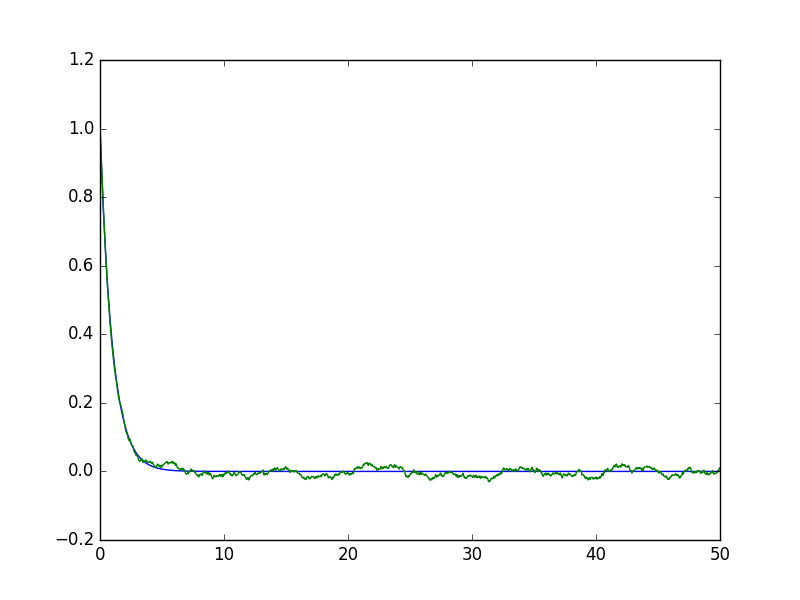
\includegraphics[width=\textwidth,
keepaspectratio]{ex6_C0_dft_cov.png}
\end{minipage}
\hspace{4mm}
\begin{minipage}[c]{.47\textwidth}
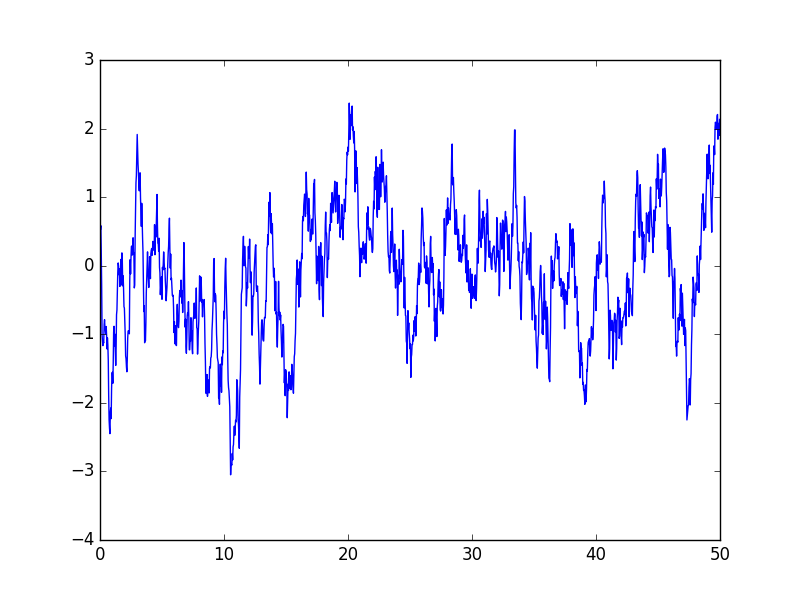
\includegraphics[width=\textwidth,
keepaspectratio]{ex6_C0_dft_sample.png}
\end{minipage}
\caption{ \label{figure:ex6_C0_dft} Plot of the estimated covariance function (left) and of one sample of the random process (right), for the covariance function $C_0(t) = e^{-\abs{t}}$, using Fourier transform method.}
\end{figure}

\begin{figure}[htbp]
\centering
\begin{minipage}[c]{.47\textwidth}
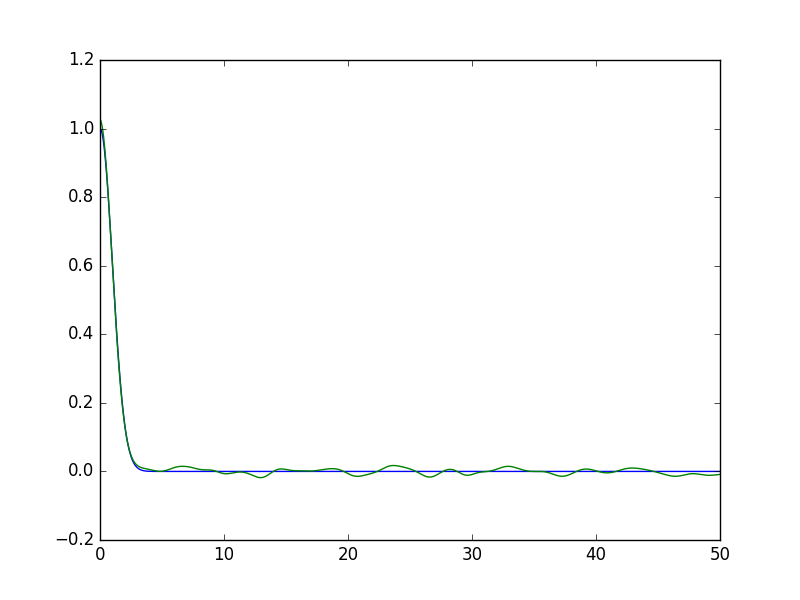
\includegraphics[width=\textwidth,
keepaspectratio]{ex6_C1_dft_cov.png}
\end{minipage}
\hspace{4mm}
\begin{minipage}[c]{.47\textwidth}
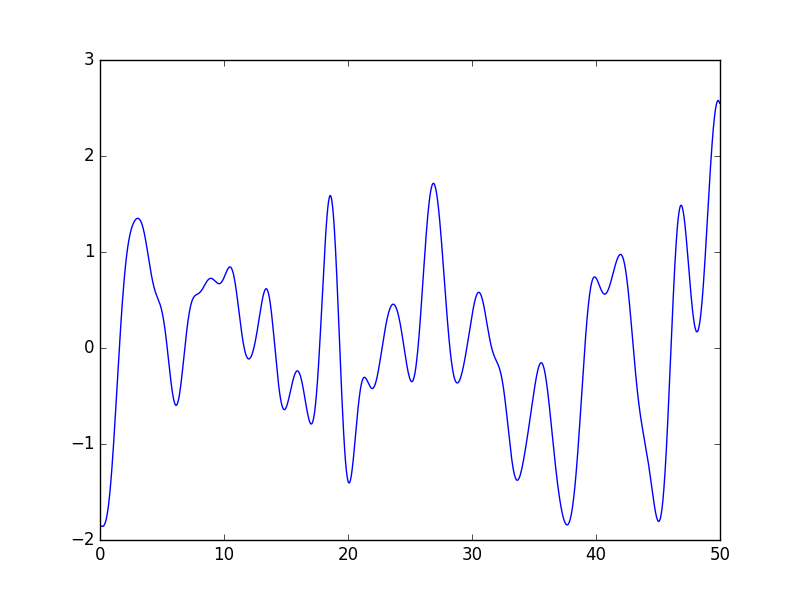
\includegraphics[width=\textwidth,
keepaspectratio]{ex6_C1_dft_sample.png}
\end{minipage}
\caption{ \label{figure:ex6_C1_dft} Plot of the estimated covariance function (left) and of one sample of the random process (right), for the covariance function $C_1(t) = e^{-t^2/2}$, using Fourier transform method.}
\end{figure}

\begin{figure}[htbp]
\centering
\begin{minipage}[c]{.47\textwidth}
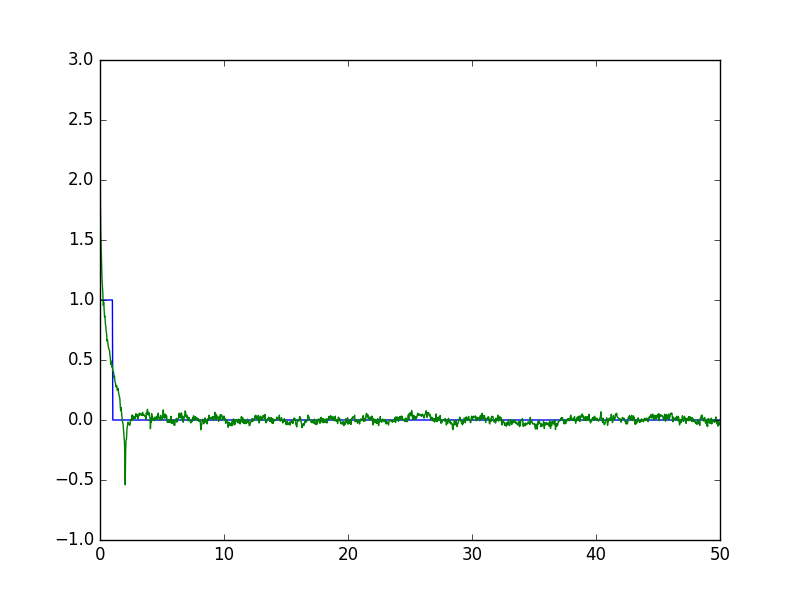
\includegraphics[width=\textwidth,
keepaspectratio]{ex6_C2_dft_cov.png}
\end{minipage}
\hspace{4mm}
\begin{minipage}[c]{.47\textwidth}
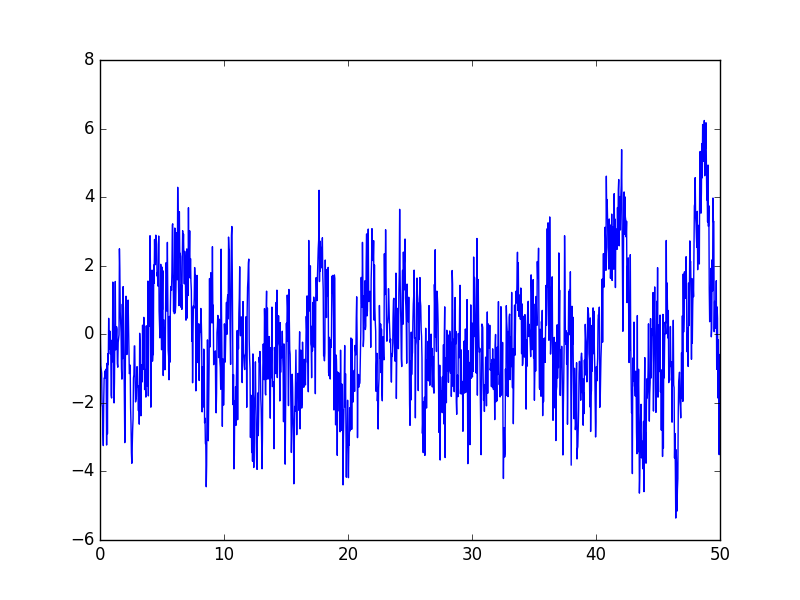
\includegraphics[width=\textwidth,
keepaspectratio]{ex6_C2_dft_sample.png}
\end{minipage}
\caption{ \label{figure:ex6_C2_dft} Plot of the estimated covariance function (left) and of one sample of the random process (right), for the covariance function $C_2(t) = \mathbbm{1}_{\bra{\abs{t}\leq1}}$, using Fourier transform method.}
\end{figure}

\paragraph*{(d)} It is easy to notice from Figures \ref{figure:ex6_C0_dft}, \ref{figure:ex6_C1_dft},  \ref{figure:ex6_C2_dft}, that the smoother the covariance function, the smoother the generated random field is. This is perfectly in accordance with what we said in Ex. 2-(d).

\paragraph*{(e)} Finally, we tried to generate the same random processes and to compute their estimate covariance by using the method based on Cholesky decomposition of the covariance matrix, as explained in HW 5, Ex. 2. In the attached \texttt{python} we wrote the function to do this as well. What we find when we try to run this function is that it works well, as long as the covariance function we are considering provides a (numerically) definite positive covariance matrix. In our case, it works well for the covariance function $C_0(t)$, but it fails for the covariance function $C_1(t)$, $C_2(t)$, due non-definite positiveness (numerical in case of $C_1$) of the covariance matrix.
In Figure \ref{figure:ex6_C0_chol} we plotted the estimation of the covariance function (versus the real one) and one sample of the random process, for the covariance function $C_0$, using the Cholesky method. 

\begin{figure}[htbp]
\centering
\begin{minipage}[c]{.47\textwidth}
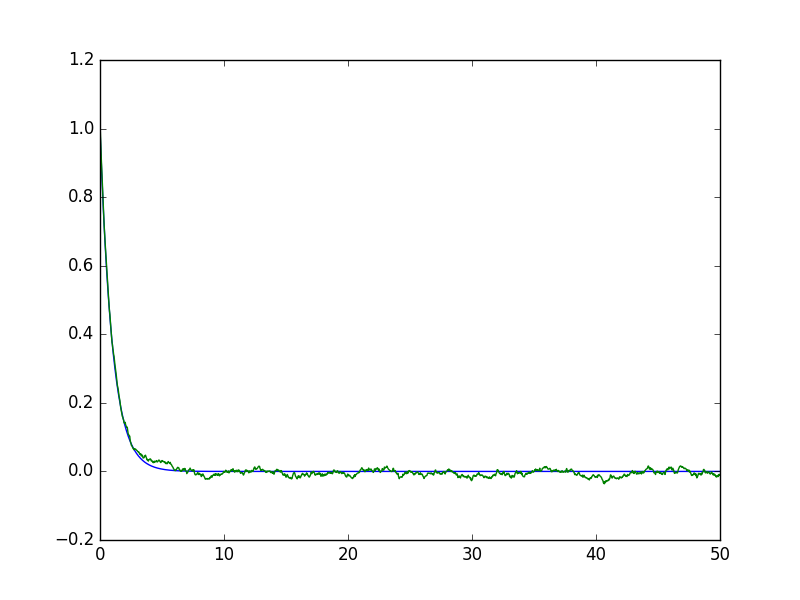
\includegraphics[width=\textwidth,
keepaspectratio]{ex6_C0_chol_cov.png}
\end{minipage}
\hspace{4mm}
\begin{minipage}[c]{.47\textwidth}
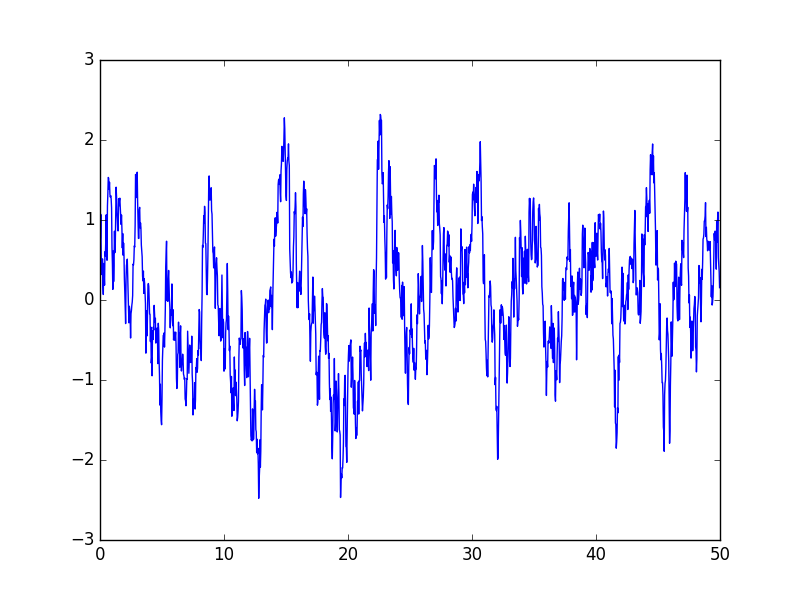
\includegraphics[width=\textwidth,
keepaspectratio]{ex6_C0_chol_sample.png}
\end{minipage}
\caption{ \label{figure:ex6_C0_chol} Plot of the estimated covariance function (left) and of one sample of the random process (right), for the covariance function $C_0(t) = e^{-\abs{t}}$, using Cholesky method.}
\end{figure}

What we just said is true as long as we use the same $L,N$ of part (c); changing them can make the method work. Therefore I think that we can say that the Cholesky method is a better choice (since it is faster than the Fourier transform method and it achieves the same accuracy) but it is not always usable, this heavily depending on the covariance function we are considering. I think that this problem could probably be fixed using the SVD decomposition instead 
of the Cholesky one.

\end{document}